\section{Spielablauf}
\label{sec:spielwelt-regeln}

\autorbeginn{Britta}

Der idealtypische Verlauf von Star Greg lässt in vier Phasen unterteilen (vgl. \ref{fig:ablaufbild}). Anhand der Beschreibung eines beispielhaften Rundenverlaufs wird dargestellt, was in den einzelnen Phasen geschieht und was der Spieler entscheiden kann.

\begin{figure}[htb]
\centering
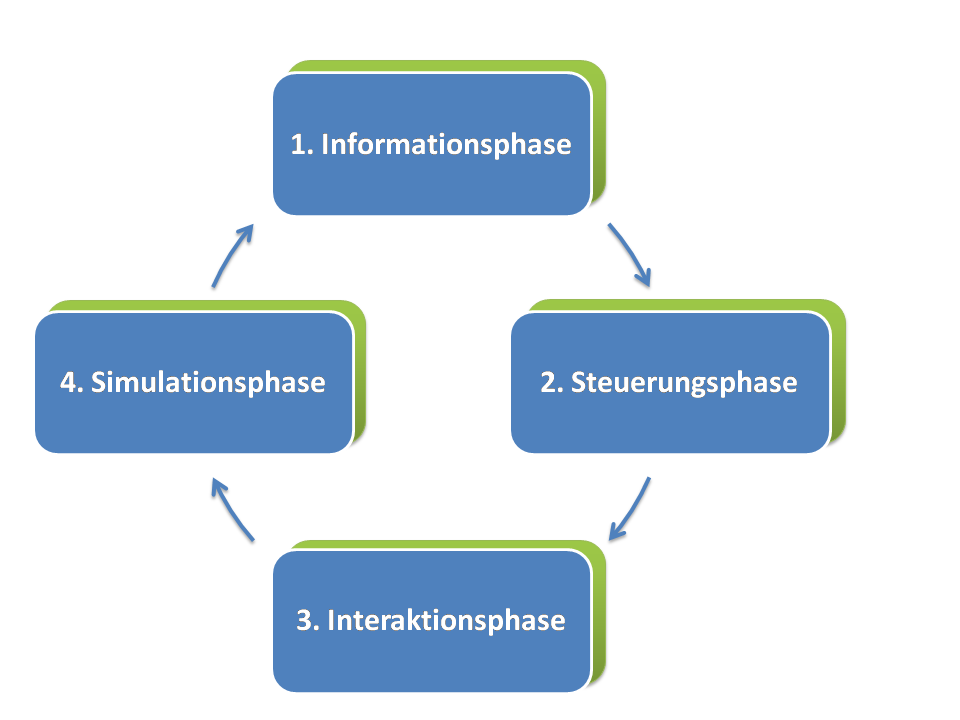
\includegraphics[width=0.75\textwidth]{20_Spielwelt/40_Regeln_Ablauf/Spielablauf.png}
\caption{Spielablauf}\label{fig:ablaufbild}
\end{figure}



\subsection{Einleitung}
\label{sub:spielwelt-datenbasis-einleitung}

\subsubsection{Flexibilität der Datenbasis}
\label{subsub:spielwelt-datenbasis-einleitung-fleibilität}

Da die Auswirkungen der Standardwerte auf den gesamten Spielverlauf im Vorhinein eines ersten Spieltests kaum absehbar sind, muss gewährleistet sein, dass die Werte innerhalb der Projektdurchführung angepasst werden können. Auch verworfene oder neue Ideen bringen oft eine Veränderung der Werte mit sich, weshalb auch hier die Notwendigkeit der Flexibiltät gegeben ist.


\subsubsection{Flexibilität der Datenbasis}
\label{subsub:spielwelt-datenbasis-einleitung-fleibilität}

Da die Auswirkungen der Standardwerte auf den gesamten Spielverlauf im Vorhinein eines ersten Spieltests kaum absehbar sind, muss gewährleistet sein, dass die Werte innerhalb der Projektdurchführung angepasst werden können. Auch verworfene oder neue Ideen bringen oft eine Veränderung der Werte mit sich, weshalb auch hier die Notwendigkeit der Flexibiltät gegeben ist.



\subsection{Einleitung}
\label{sub:spielwelt-datenbasis-einleitung}

\subsubsection{Flexibilität der Datenbasis}
\label{subsub:spielwelt-datenbasis-einleitung-fleibilität}

Da die Auswirkungen der Standardwerte auf den gesamten Spielverlauf im Vorhinein eines ersten Spieltests kaum absehbar sind, muss gewährleistet sein, dass die Werte innerhalb der Projektdurchführung angepasst werden können. Auch verworfene oder neue Ideen bringen oft eine Veränderung der Werte mit sich, weshalb auch hier die Notwendigkeit der Flexibiltät gegeben ist.


\subsubsection{Flexibilität der Datenbasis}
\label{subsub:spielwelt-datenbasis-einleitung-fleibilität}

Da die Auswirkungen der Standardwerte auf den gesamten Spielverlauf im Vorhinein eines ersten Spieltests kaum absehbar sind, muss gewährleistet sein, dass die Werte innerhalb der Projektdurchführung angepasst werden können. Auch verworfene oder neue Ideen bringen oft eine Veränderung der Werte mit sich, weshalb auch hier die Notwendigkeit der Flexibiltät gegeben ist.



\subsection{Einleitung}
\label{sub:spielwelt-datenbasis-einleitung}

\subsubsection{Flexibilität der Datenbasis}
\label{subsub:spielwelt-datenbasis-einleitung-fleibilität}

Da die Auswirkungen der Standardwerte auf den gesamten Spielverlauf im Vorhinein eines ersten Spieltests kaum absehbar sind, muss gewährleistet sein, dass die Werte innerhalb der Projektdurchführung angepasst werden können. Auch verworfene oder neue Ideen bringen oft eine Veränderung der Werte mit sich, weshalb auch hier die Notwendigkeit der Flexibiltät gegeben ist.


\subsubsection{Flexibilität der Datenbasis}
\label{subsub:spielwelt-datenbasis-einleitung-fleibilität}

Da die Auswirkungen der Standardwerte auf den gesamten Spielverlauf im Vorhinein eines ersten Spieltests kaum absehbar sind, muss gewährleistet sein, dass die Werte innerhalb der Projektdurchführung angepasst werden können. Auch verworfene oder neue Ideen bringen oft eine Veränderung der Werte mit sich, weshalb auch hier die Notwendigkeit der Flexibiltät gegeben ist.



\subsection{Einleitung}
\label{sub:spielwelt-datenbasis-einleitung}

\subsubsection{Flexibilität der Datenbasis}
\label{subsub:spielwelt-datenbasis-einleitung-fleibilität}

Da die Auswirkungen der Standardwerte auf den gesamten Spielverlauf im Vorhinein eines ersten Spieltests kaum absehbar sind, muss gewährleistet sein, dass die Werte innerhalb der Projektdurchführung angepasst werden können. Auch verworfene oder neue Ideen bringen oft eine Veränderung der Werte mit sich, weshalb auch hier die Notwendigkeit der Flexibiltät gegeben ist.


\subsubsection{Flexibilität der Datenbasis}
\label{subsub:spielwelt-datenbasis-einleitung-fleibilität}

Da die Auswirkungen der Standardwerte auf den gesamten Spielverlauf im Vorhinein eines ersten Spieltests kaum absehbar sind, muss gewährleistet sein, dass die Werte innerhalb der Projektdurchführung angepasst werden können. Auch verworfene oder neue Ideen bringen oft eine Veränderung der Werte mit sich, weshalb auch hier die Notwendigkeit der Flexibiltät gegeben ist.





\autorende{}